Given that the real-world datasets are often noisy and the ground truths regarding the feature contributions are not known.
To address this issue, synthetic simulated datasets are used.
The goal of the simulation is to create datasets with known dependencies between the features and target variables, which can be used for evaluation.

The reason for this is to imitate multiple real-world scenarios where the relationships between the features and the target variable are different.
For instance, when examining the dataset from the M5 forecasting competition\footnote{M5 Forecasting - Accuracy dataset: \url{https://www.kaggle.com/c/m5-forecasting-accuracy/data}\label{m5ds}}, various types of time series can be identified.
Figure~\ref{fig:m5_dataset} illustrates a sample pair of household item series, where a distinct resemblance between them is noticeable.
Items with consistent demand, such as cleaning supplies and staple foods, generally exhibit similar trends.
Other datasets like the one for \emph{Store Item Demand Forecasting Challenge}\footnote{Store Item Demand Forecasting Challenge dataset: \url{https://www.kaggle.com/competitions/demand-forecasting-kernels-only/data}\label{kaggleds}}
shown on the Fig.~\ref{fig:datasets} have multiple series with different seasonal patterns of the target variable.
Products such as ice-cream and sun cream are typically aligned with this seasonal trend.


\begin{figure}[t]
    \centering
    \begin{subfigure}[t]{0.45\textwidth}
        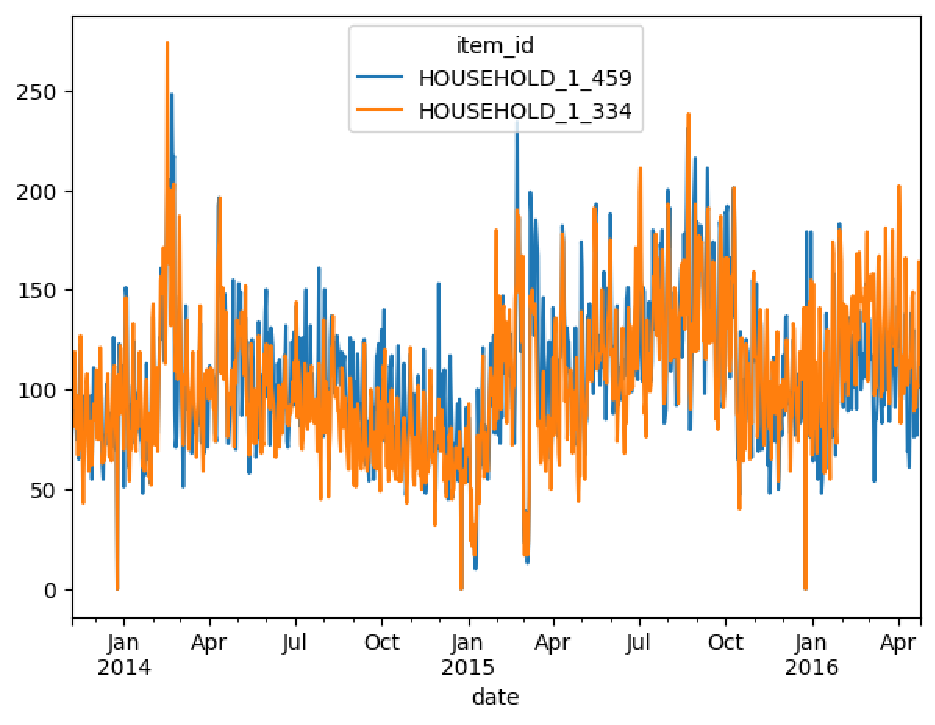
\includegraphics[width=\textwidth]{chapters/04_feature_importance_estimation/img/m5_lin}
        \caption{M5 Forecasting - Accuracy dataset samples \ref{m5ds}}
        \label{fig:m5_dataset}
    \end{subfigure} %
    ~%
    \begin{subfigure}[t]{0.45\textwidth}
        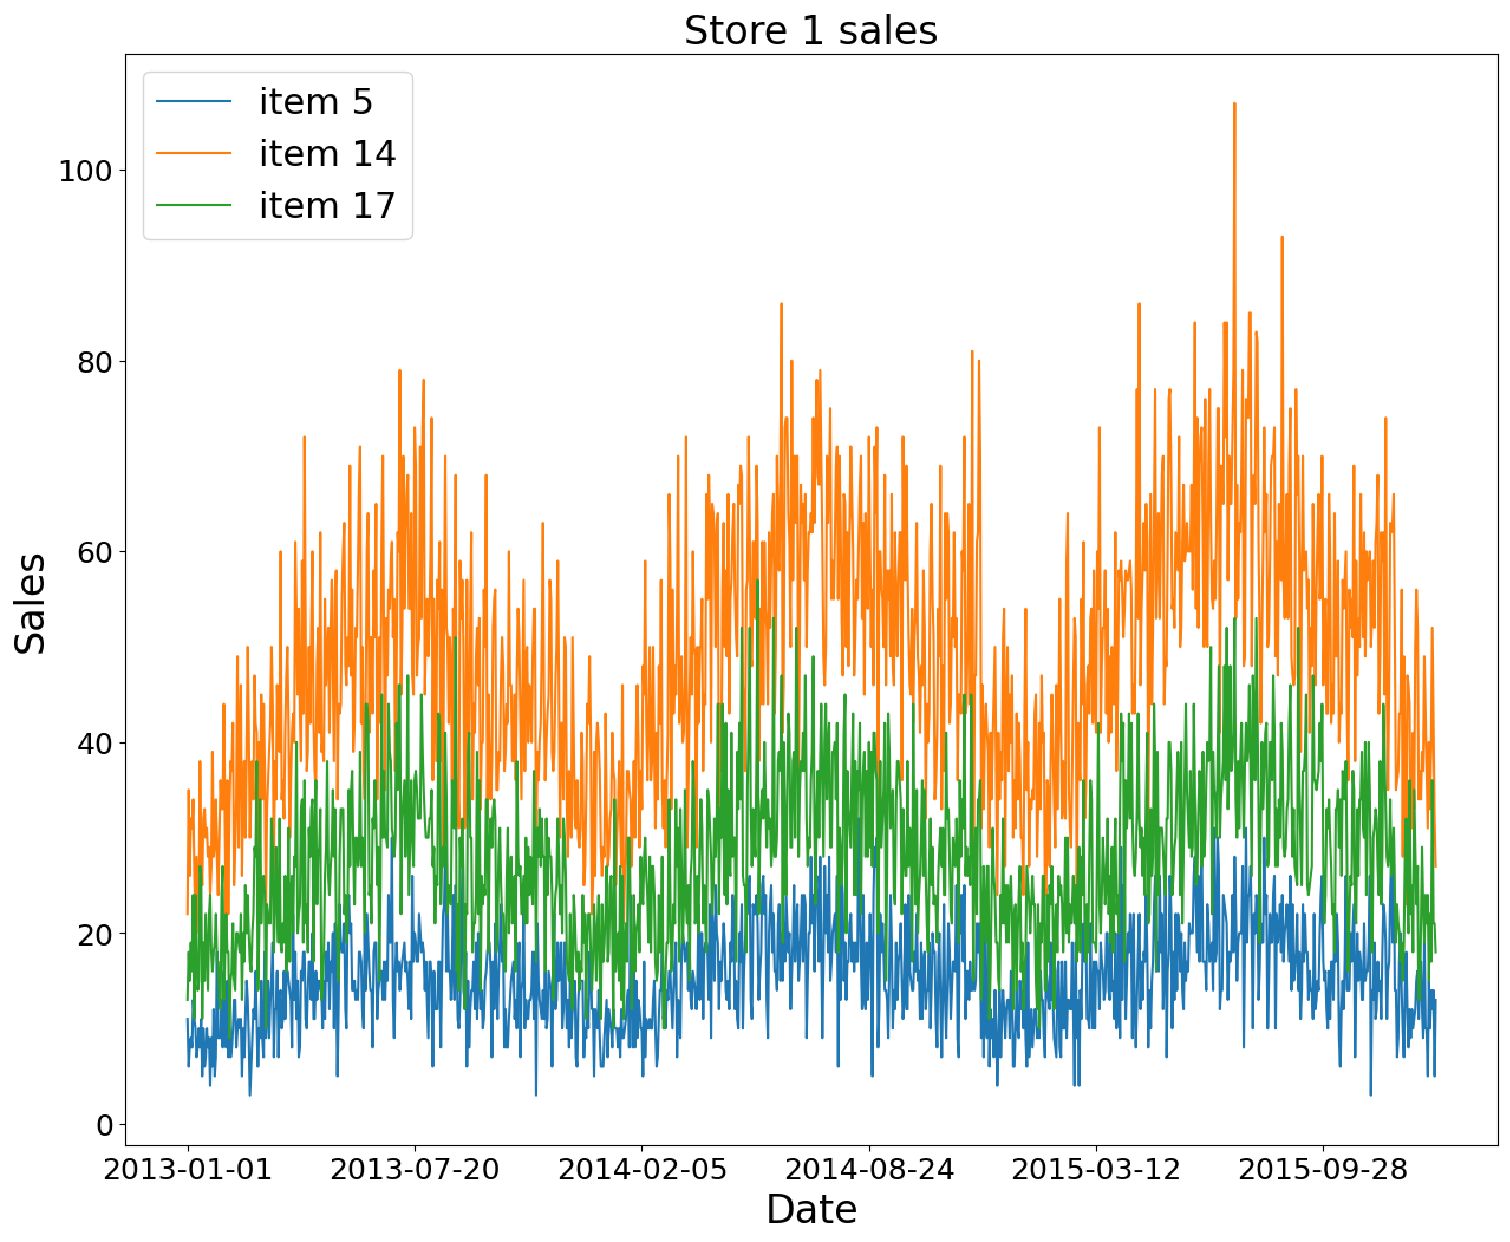
\includegraphics[width=\textwidth]{chapters/04_feature_importance_estimation/img/kaggle_demand}
        \caption{Store Item Demand Forecasting \\ Challenge dataset samples \ref{kaggleds}}
        \label{fig:kaggle_dataset}
    \end{subfigure}
    \caption{Example datasets for demand forecasting problems}
    \label{fig:datasets}
\end{figure}

Based on these example datasets, two data generation processes were developed: one linear and one non-linear.

\subsubsection[Linear data simulation] {Linear data simulation}
\label{sec:linear_data_simulation}


%Autoregressive model for linear data simulation was used to generate the dataset.
%\textcolor{red}{Describe the process of generating the linear data.}

The linear data generation process consists of:
i) Lag features: $x_{t-1},  ..., x_{t-n}$ are $n$ lagged variables of the target variable, ii) External demand drivers: $ex_1, ex_2, ..., ex_n$ are external factors that influence the target variable, and iii) Noise: $\epsilon$ is the noise term.
To obtain multiple time series which are related, we extend the linear data generation process to include a series-scaling factor $s$ and a base demand $b$.
By using the base demand and scaling factor we can initialize the data generation process for each series with different values.
The scaling factor was not used on the lagged variables as they are already scaled by the target variable.
The final formula for the linear data generation process is the following:
$$
x_t = \beta_1 x_{t-1} + ... + \beta_n x_{t-n} + s \cdot ( ex_1 + .. ex_n + b + \epsilon)
$$




For the linear data generation process, two lagged variables with $\beta_{1,2} = [0.6,0.2]$ weights were used.
As exogenous variables, two additional features were generated, one representing a holiday effect present or not given by a binary random variable, and an additional external factor called temperature with a normal distribution $N(20,5)$.
Over the result, scaling factors $s_{1,2,3} = [0.5,1,2]$ were applied, with base demand $b=100$ and noise $\epsilon = \mathcal{N}(1,0.05)$.
The concrete example is shown in Fig.~\ref{fig:linear_data_generation}.
Inspecting the partial autocorrelation of the time series in Fig.~\ref{fig:partialautocorrelation} it can be observed that the first two lags have the highest value, meaning that the first two lags explain most of the variance.

\begin{figure}[t]
    \centering
    \begin{subfigure}[t]{0.45\textwidth}
        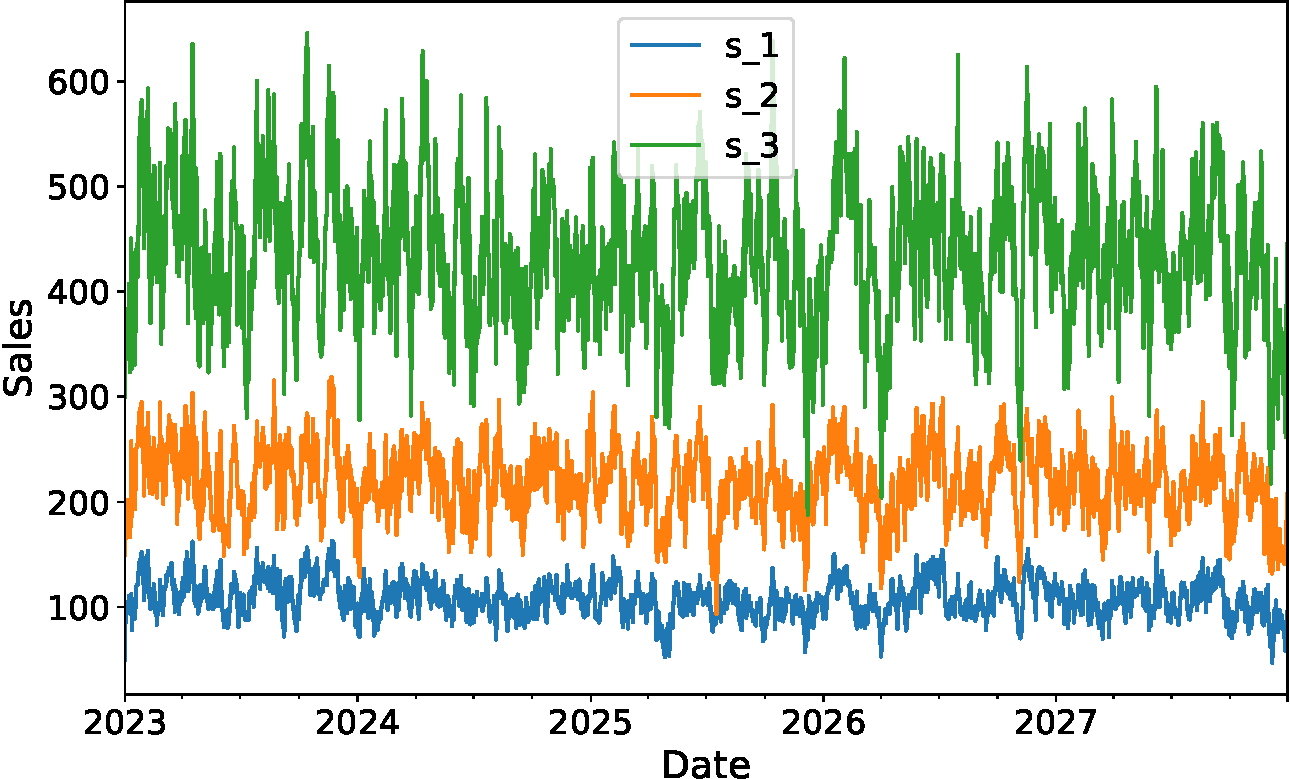
\includegraphics[width=\textwidth]{chapters/04_feature_importance_estimation/img/linear_dep_time_series}
        \caption{Linear data generation process example of 3 series with scaling $s_{1,2,3} = [0.5,1,2]$ , base demand $b=100$}
        \label{fig:linear_data_generation}
    \end{subfigure}%
    \hfill
    \begin{subfigure}[t]{0.45\textwidth}
        \centering
        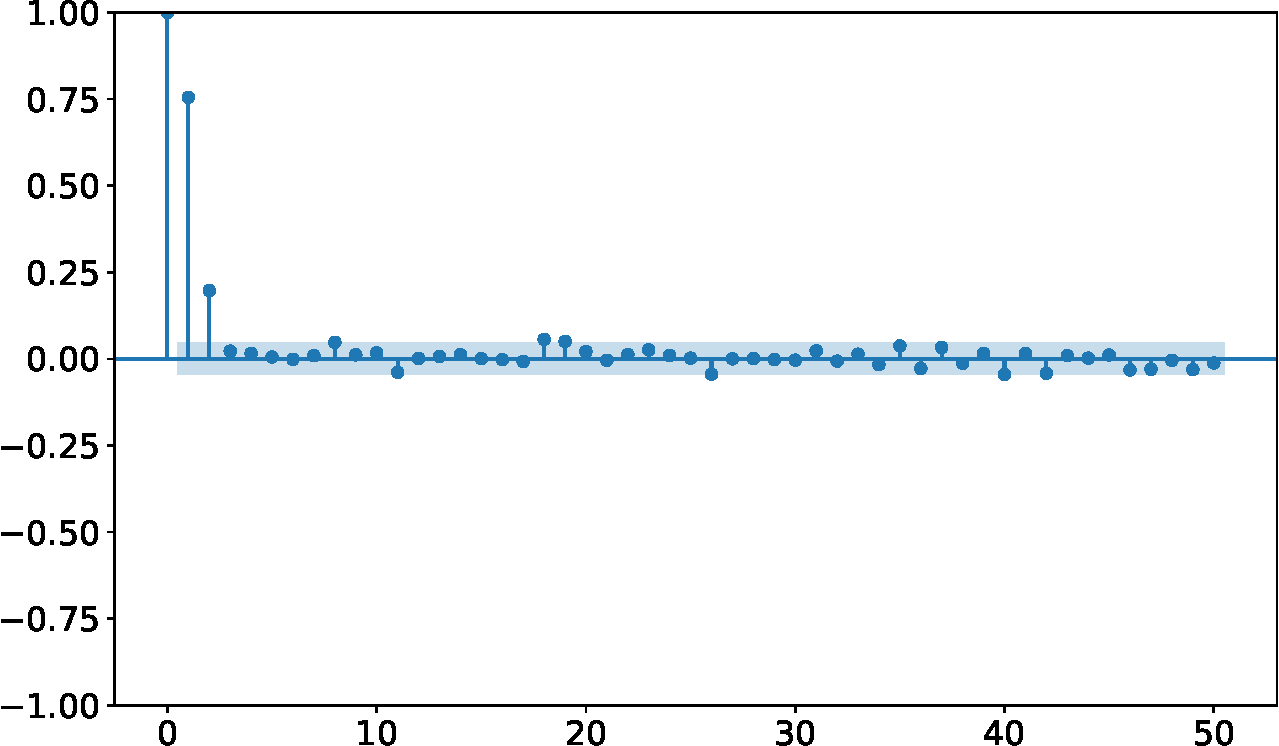
\includegraphics[width=\textwidth]{chapters/04_feature_importance_estimation/img/linear_dep_time_series_acf_pacf_s_1}
        \caption{Partial autocorrelation of lagged variable for series 1}
        \label{fig:partialautocorrelation}
    \end{subfigure}
    \caption{Linear data generation process}
\end{figure}

\subsubsection{Non-linear data simulation}
\label{sec:non-linear-data-simulation}


Similarly, to the linear data generation, the non-linear data generation consists of the following components.
The basis of the data generation is a seasonal trend $S = A \cdot sin(P)$ where $A$ denotes the amplitude and $P= (2 \cdot \pi)/365$ (365 days) is the period. To this we add a holiday effect $H$, a weekend effect $W$, a scaling factor $s_{1,2,3}$, and noise $\epsilon$. The base demand $b$ is also included in the formula.
The final formula for the non-linear data generation process is:
$$
x_t = s \cdot S \cdot H \cdot W \cdot \epsilon \cdot b
$$


To generate the dataset, with the non-linear feature contributions, an additional time series generator library\footnote{Time Series Generator - \url{http://https://github.com/Nike-Inc/timeseries-generator}\label{timeseries-generator}} was used.
The following components were used to generate the data, scaling $s_{1,2,3} = [0.5,1,2]$, base demand $b=100$, noise $\epsilon = \mathcal{N}(1,0.05)$, holiday effect $H=1.5$ with fade-in and out effect and seasonality $S = A * sin(P)$ where $A_{1,2,3} = [0.2,0.3,0.4]$ and weekend effect $W = 1.3$ if weekend, $1$ otherwise.
The concrete example is shown in Fig. \ref{fig:nonlinear_data_generation}.

\begin{figure}[t]
    \centering
    \begin{subfigure}[t]{0.45\textwidth}
        \centering
        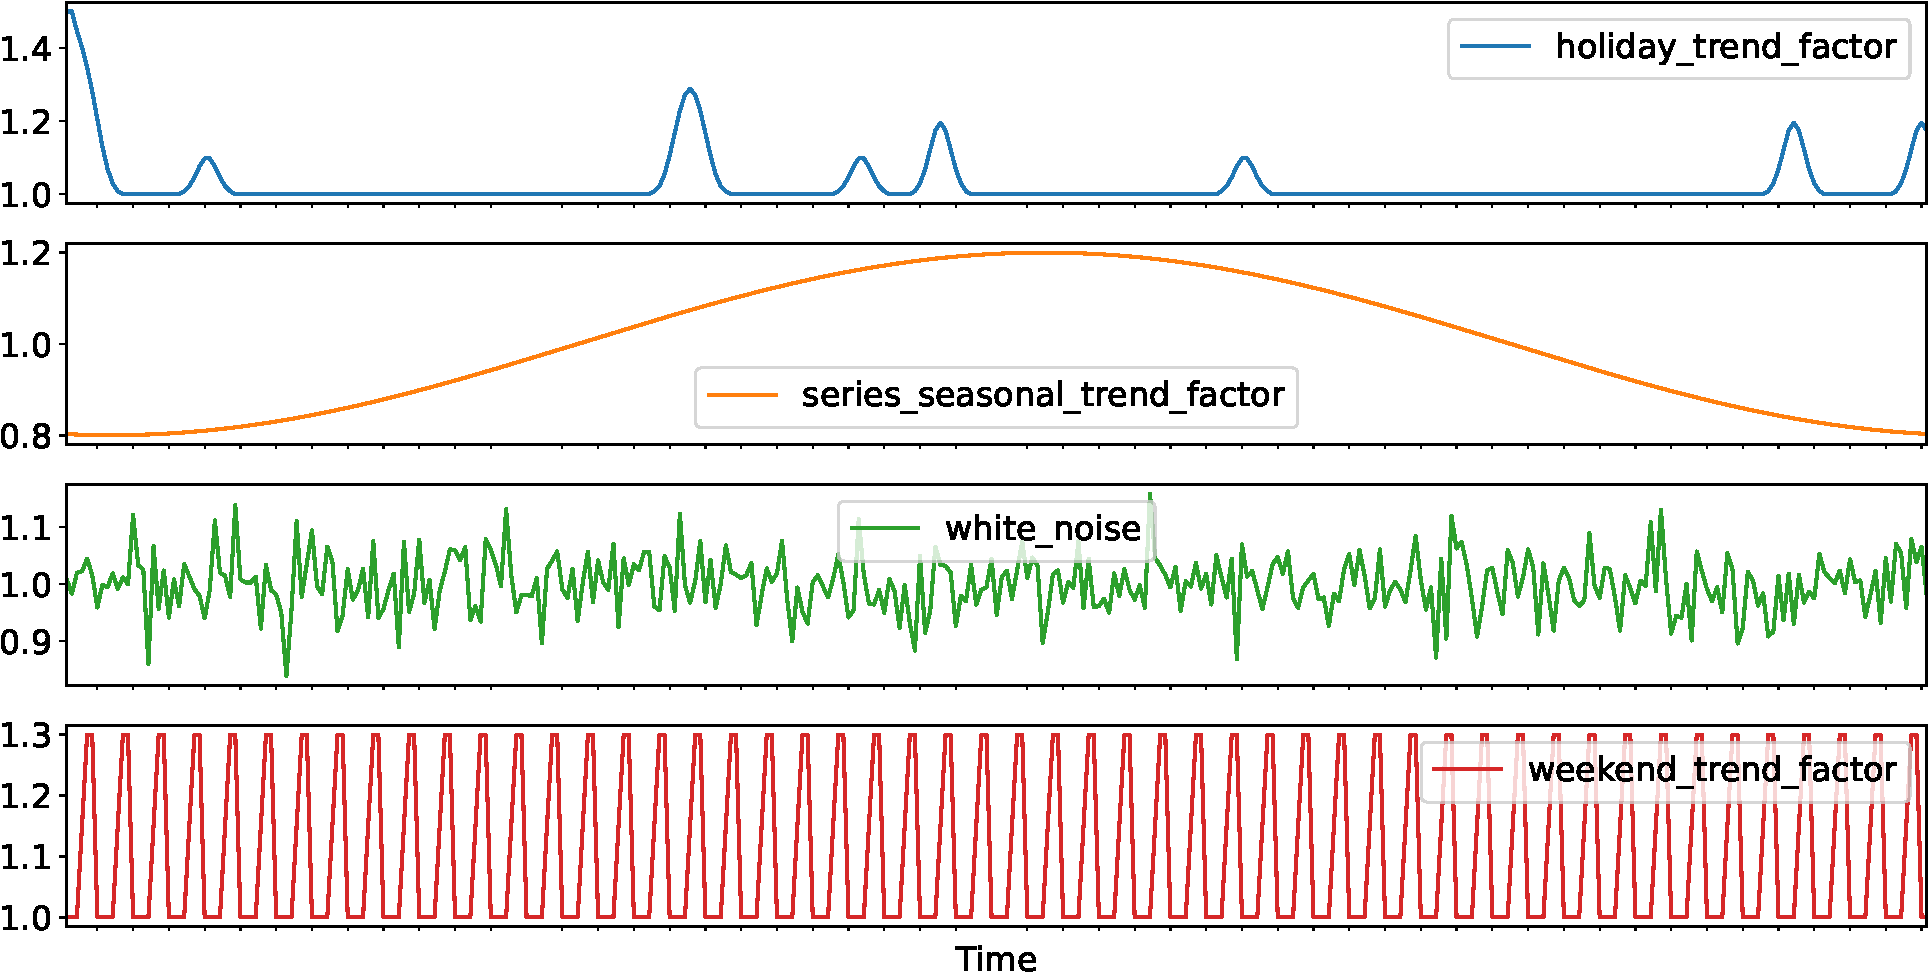
\includegraphics[width=\textwidth]{chapters/04_feature_importance_estimation/img/non_linear_time_series_components}
        \caption{Components of the non-linear data generation process}
        \label{fig:nonlinear_data_generation_components}
    \end{subfigure}
    \hfill
    \begin{subfigure}[t]{0.45\textwidth}
        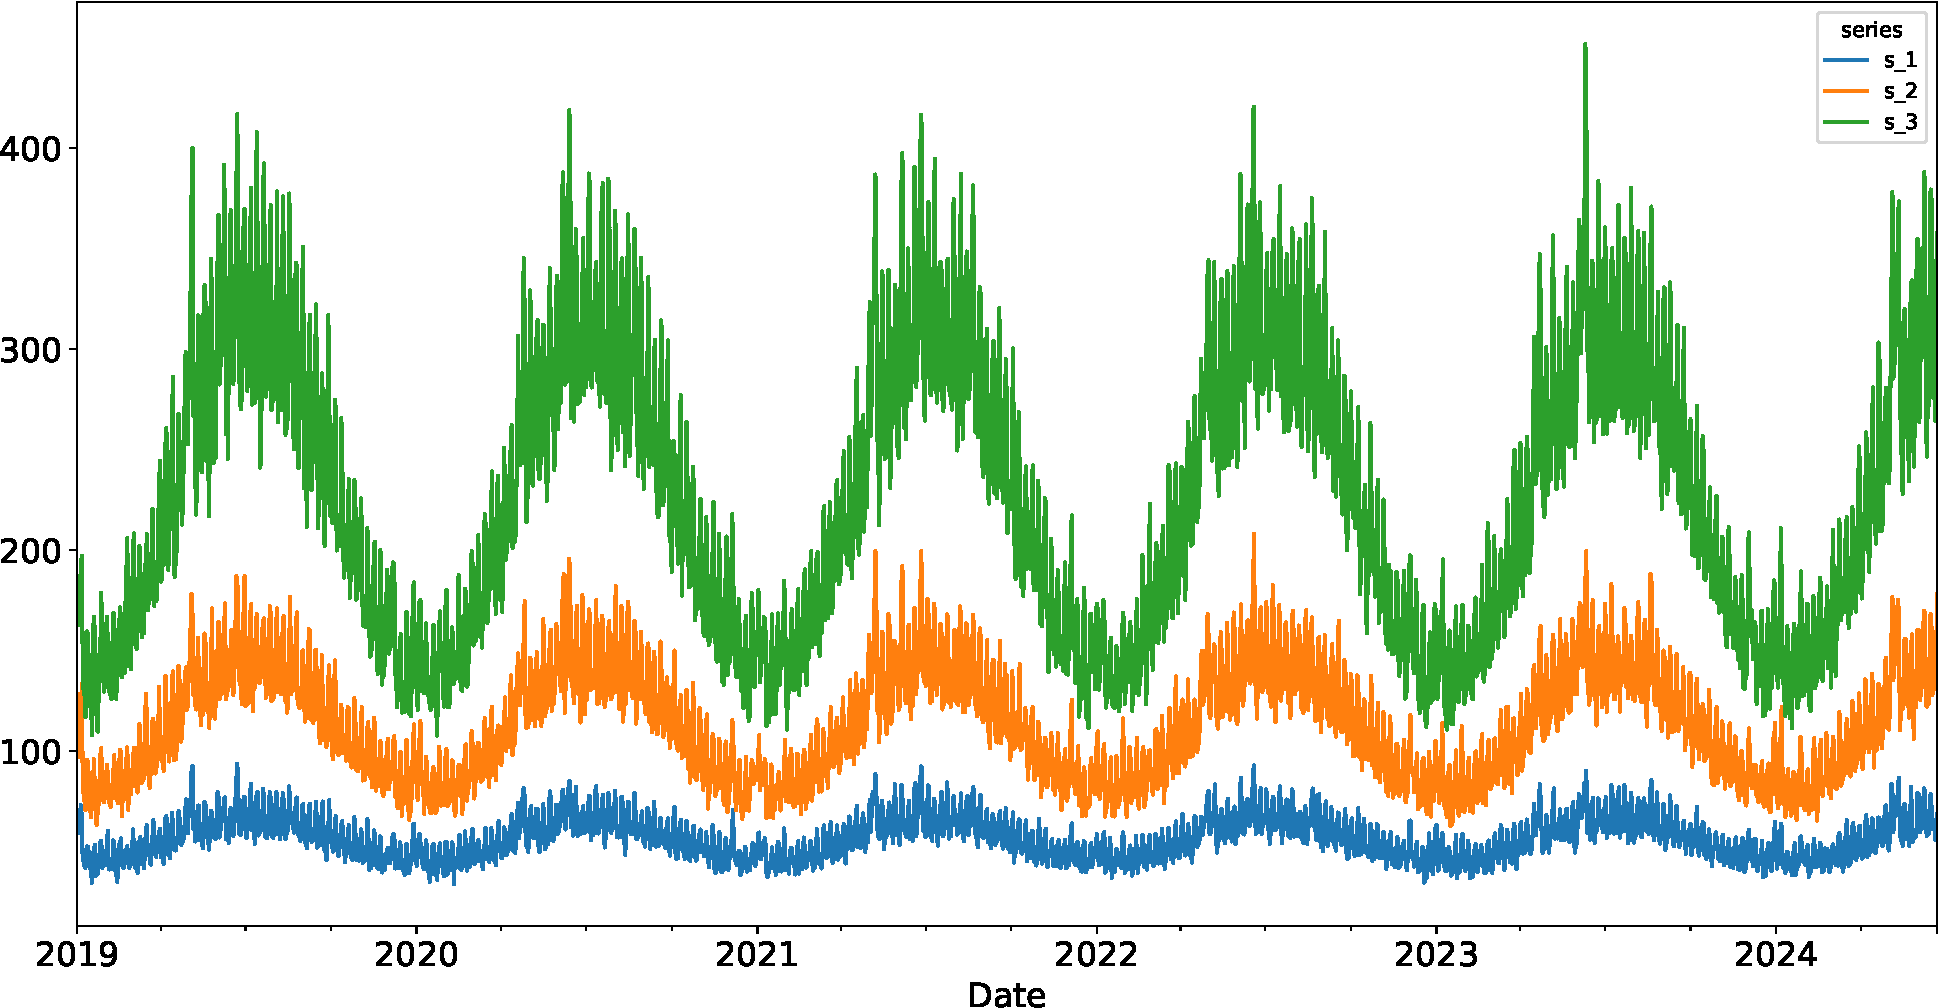
\includegraphics[width=\textwidth]{chapters/04_feature_importance_estimation/img/non_linear_time_series}
        \caption{Non-linear data generation process of 3 series with scaling $s_{1,2,3} = [0.5,1,2]$ , base demand $b=100$ }
        \label{fig:nonlinear_data_generation}
    \end{subfigure}
    \caption{Non-linear data generation process}
\end{figure}

%The dataset obtained seasonal autorergressive model with exogenous variables (SARIMAX) .